\clearpage
\appendix
\begingroup
\renewcommand{\chaptername}{Appendix}
\titleformat{\chapter}[hang]{\normalfont\bfseries\Large}{\chaptername\ \thechapter.}{0.5em}{}
\titlespacing*{\chapter}{0pt}{0pt}{12pt}
\addtocontents{toc}{\protect\renewcommand{\protect\cftchappresnum}{Appendix~}}

\begin{landscape}
\chapter{Comprehensive Master Schematic of the RC-Free Pipeline}
\label{app:master-pipeline}
\begin{figure}[H]
\centering
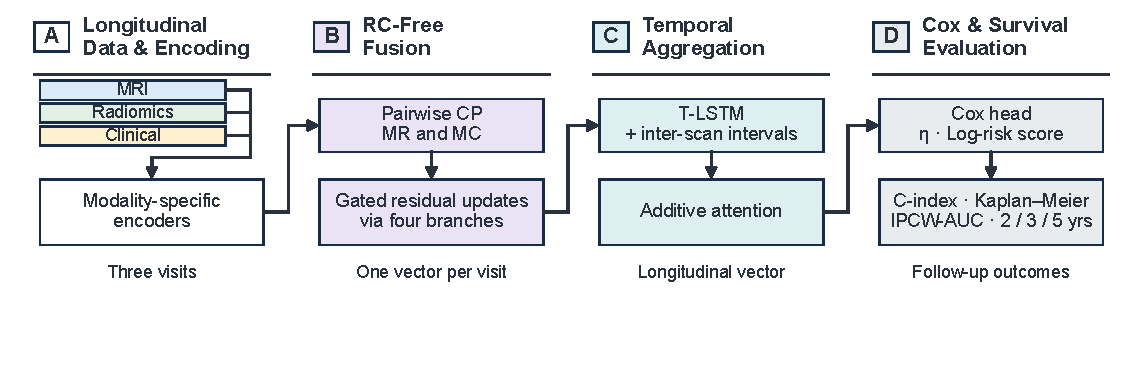
\includegraphics[width=\linewidth,height=11.5cm,keepaspectratio]{image_en/master-pipeline.pdf}
\caption{End-to-end master schematic of the RC-Free pipeline from raw inputs to survival evaluation}
\label{fig:master-pipeline}
\end{figure}
\end{landscape}

\clearpage
\chapter{Feature Map Dimensions of the 3D MRI Encoder}
\label{app:mri-shapes}
Table~\ref{tab:mri-encoder-shapes} details the intermediate feature map dimensions across each stage of the 3D ResNet-18 MRI encoder (implemented in MONAI version 1.5.2 and initialized from MedicalNet pretrained weights \cite{chen2019med3d,cardoso2022monai}). Each 3D feature map has shape $[B, C_{\mathrm{ch}}, D, H, W]$, where $B$ denotes the batch size, $C_{\mathrm{ch}}$ denotes the number of channels, and $D, H, W$ represent the three spatial dimensions. All three visits of a participant share this encoder; following global average pooling, the three 512-dimensional vectors are stacked along the temporal axis into $[B, 3, 512]$ before being linearly projected to $M_t\in\mathbb R^{128}$.

\begin{table}[H]
\centering
\small
\caption[Feature map dimensions of the 3D ResNet-18 encoder]{Feature map dimensions across layers of the 3D ResNet-18 volumetric encoder}
\label{tab:mri-encoder-shapes}
\begin{tabularx}{\textwidth}{@{}Y l@{}}
\toprule
\textbf{Stage / Operation} & \textbf{Output Shape} \\
\midrule
Input 3D MRI volume & $[B,1,144,144,144]$ \\
$7^3$ 3D convolution, stride 1, padding 3; BN; ReLU & $[B,64,144,144,144]$ \\
$3^3$ max pooling, stride 2, padding 1 & $[B,64,72,72,72]$ \\
ResNet Stage 1: two BasicBlocks & $[B,64,72,72,72]$ \\
ResNet Stage 2: first block stride 2 & $[B,128,36,36,36]$ \\
ResNet Stage 3: first block stride 2 & $[B,256,18,18,18]$ \\
ResNet Stage 4: first block stride 2 & $[B,512,9,9,9]$ \\
Global average pooling and flattening & $[B,512,1,1,1]\to[B,512]$ \\
Temporal stacking across the three visits & $[B,3,512]$ \\
Linear projection $512\to128$; GELU; Dropout 0.20; LayerNorm & $[B,3,128]$ \\
\bottomrule
\end{tabularx}
\end{table}

\endgroup
